\subsection{Open Delta Neighborhoods}
\noindent
An open delta neighborhood of a point $x_0$ is defined as the set
\begin{equation*}
	N\left(x_0, \delta\right) = \left\{x \in \mathbb{R}^n \mid \norm{x-x_0} < \delta\right\}.
\end{equation*}

\begin{figure}[H]
	\centering
	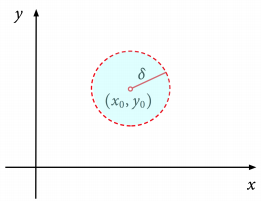
\includegraphics[width=0.5\textwidth]{./differentialMultivariableCalculus/open_delta.png}
	\caption{An open delta neighborhood centered at $(x_0, y_0)$}
\end{figure}

\noindent
This simply means all points less than a distance $\delta$ away from point $x_0$.\\
For example, $N( (1,2) , 7) = \left\{ (x,y) \mid \sqrt{(x-1)^2 + (y-2)^2}<7 \right\}$, which is a ball (filled-in circle) of radius 7 centered at $(1, 2)$.